\documentclass{article}
\usepackage[utf8]{inputenc}
\usepackage{amsmath}
\usepackage{graphicx}
\usepackage{float}
\usepackage[font=scriptsize,labelfont=bf]{caption}

\title{COMP6245 : Lab 4 Report}
\author{Thanakorn Panyapiang(tp2n19@soton.ac.uk)}
\date{}

\begin{document}
\maketitle

\section{Linear Least Square Regrssion}
The result of the linear predictors using pseudo-inverse method and using scikit-learn is shown below.
\begin{center}
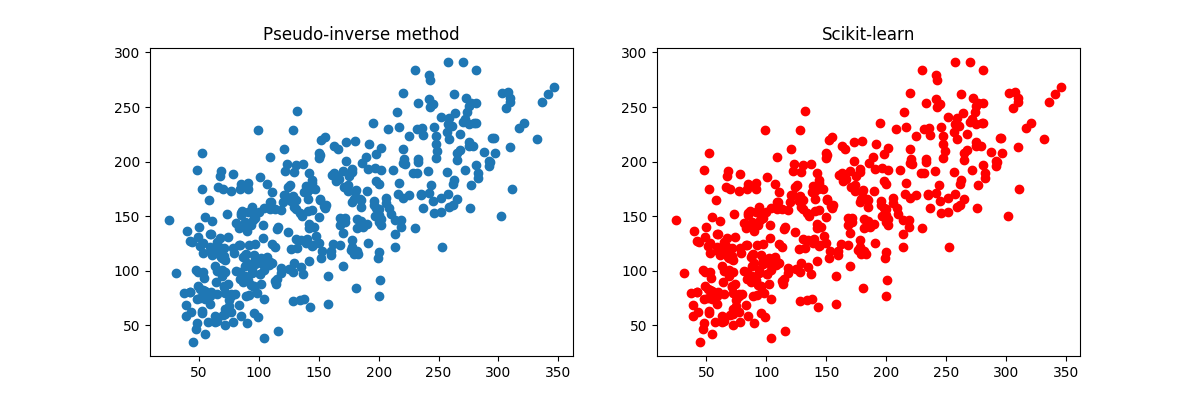
\includegraphics[scale=0.3]{diabetes_accuracy}
\end{center}
Both methods give exactly the same result as can be seen from the identical mean square error.

\section{Regularization}

The gradient of $L_{2}$ regularization can be derived as follow:
\begin{equation}
\begin{split}
	\nabla _aE_{L2} &= \frac{\partial ||f - Ya||^2_2 + \gamma ||a||^2_2}{\partial a}\\
	 &= 2Y^T(f - Ya) + 2\gamma a
\end{split}
\end{equation}
Equating the gradient to 0 gives the coefficient matrix \textit{a} as follow
\begin{equation}
\begin{split}
	0 &= 2Y^T(f - Ya) + 2\gamma a\\
	Y^TYa - \gamma a &= Y^Tf\\
	a(Y^TY - \gamma) &= Y^Tf\\
	a &= (Y^tY - \gamma)^{-1} Y^Tf 
\end{split}
\end{equation}

It can be observed that the coefficients of the predictor with $L_2$ regularization are significantly lower than the model without regularization. This is caused by adding a quadratic penalty of the weights to the error function. The coefficients of the model with and without $L_2$ regularization is shown below.
\begin{center}
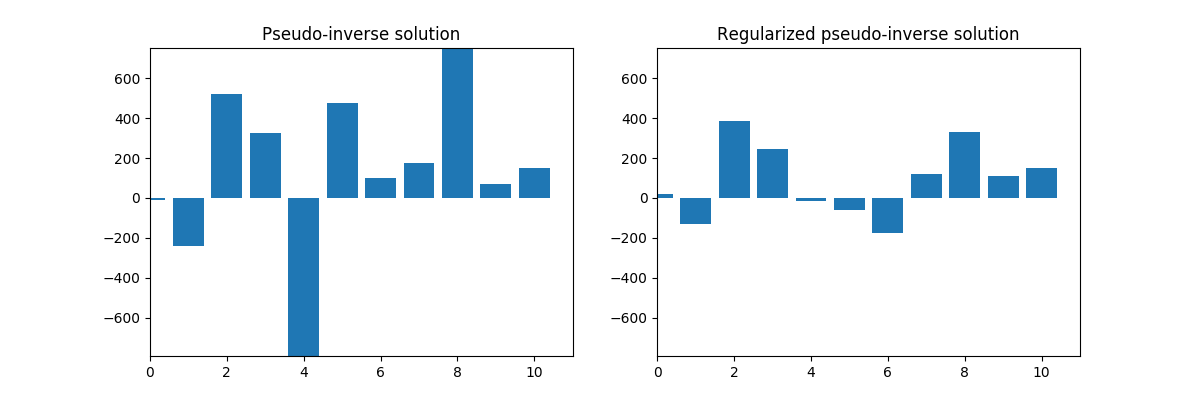
\includegraphics[scale=0.4]{reg_weights_compare}
\captionof{figure}{}
\end{center}

Moreover, when the regularization parameter($\gamma$) increases, it can be noticed that the coefficients are reduced as can be seen on Figure 2.
\begin{center}
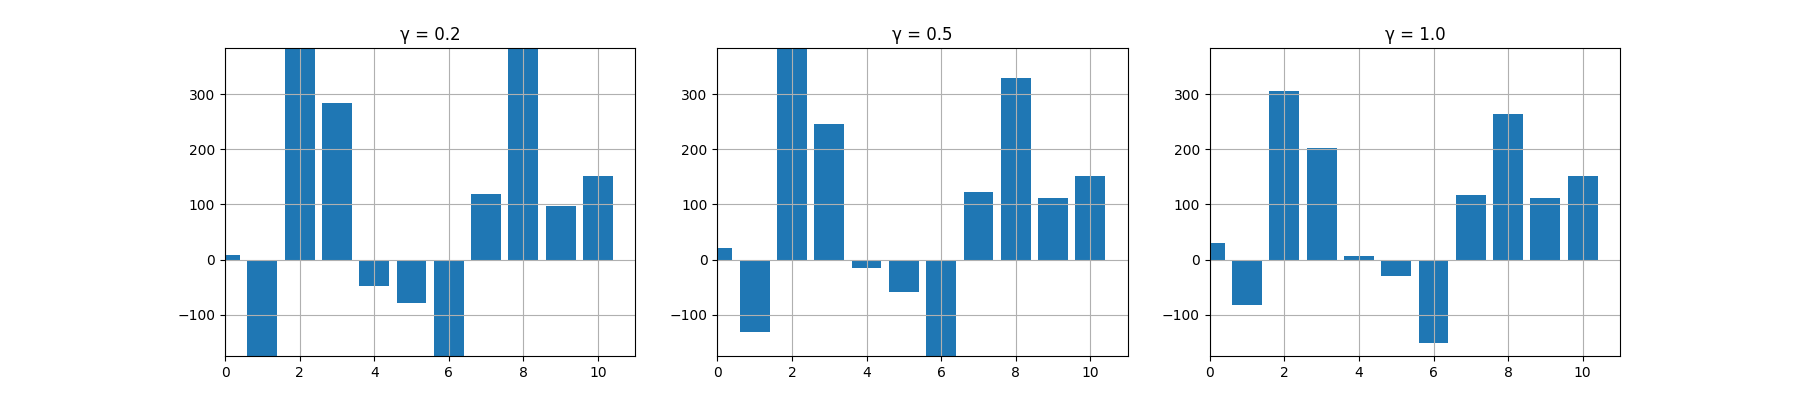
\includegraphics[scale=0.3]{ridge_weights_compare}
\captionof{figure}{}
\end{center}

\section{Sparse Regression}

The coefficients of linear regression with Lasso regularization on different $\gamma$ compare to Ridge regression is displayed in Figure 3.
\begin{center}
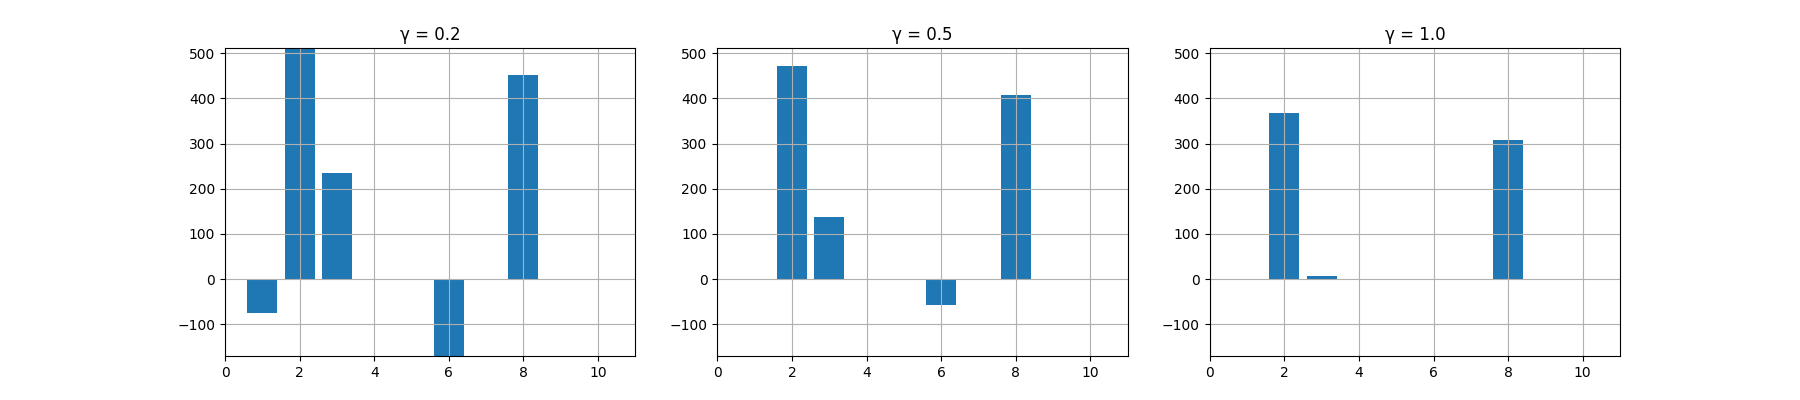
\includegraphics[scale=0.3]{lasso_compare}
\captionof{figure}{}
\end{center}

One observation on the lasso coefficients is that the numbers of zero coefficients increases along with $\gamma$.

\begin{center}
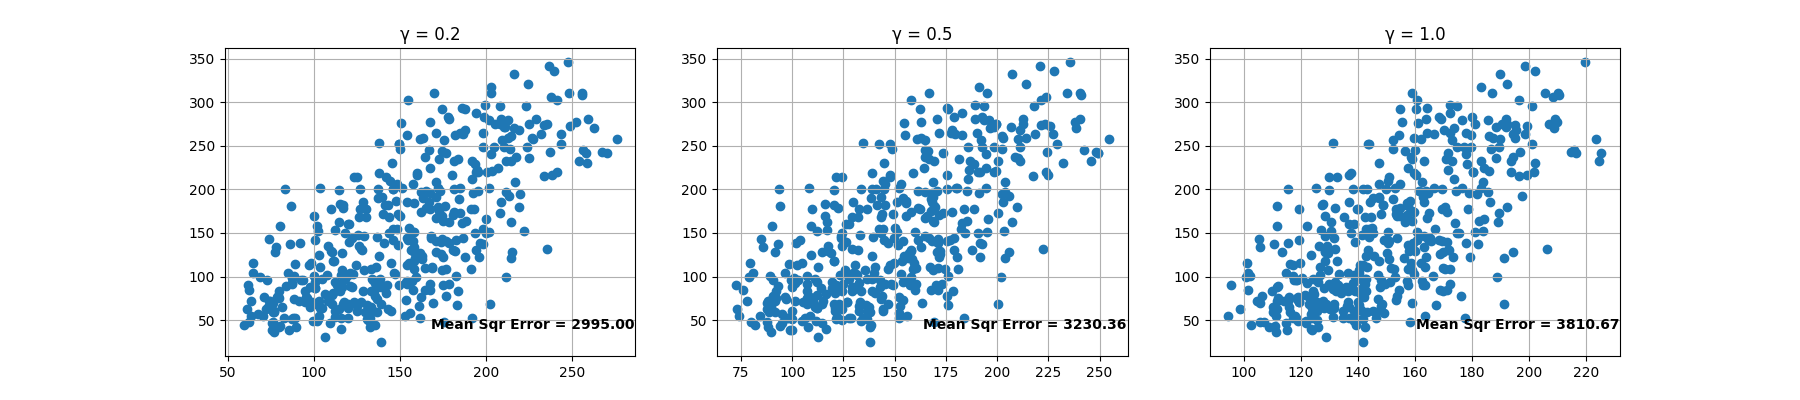
\includegraphics[scale=0.3]{lasso_error_compare}
\captionof{figure}{}
\end{center}

\indent However, this coeeficients do not indicate that the attibutes which have 0 weight are not meaningful because the prediction error goes up as the numbers of zero coefficients increases as show in Figure 4. This suggests that, for the diabetes dataset, there are more useful features than the irrelevant ones so that when several parameters are removed the prediction becomes less accurate.

Lasso removes some useful features from the model because there are some features which are correlated to each other. Therefore, in order to minimize the penalty term($\gamma||a||_1$), Lasso chooses only one of these features. From the scatter plot below, it can be noticed that the $8^{th}$ attribute, which has a non-zero coefficient, is positively correlated with the $0^{th}$ and $4^{th}$ attibutes, which have a zero coefficient.
\begin{center}
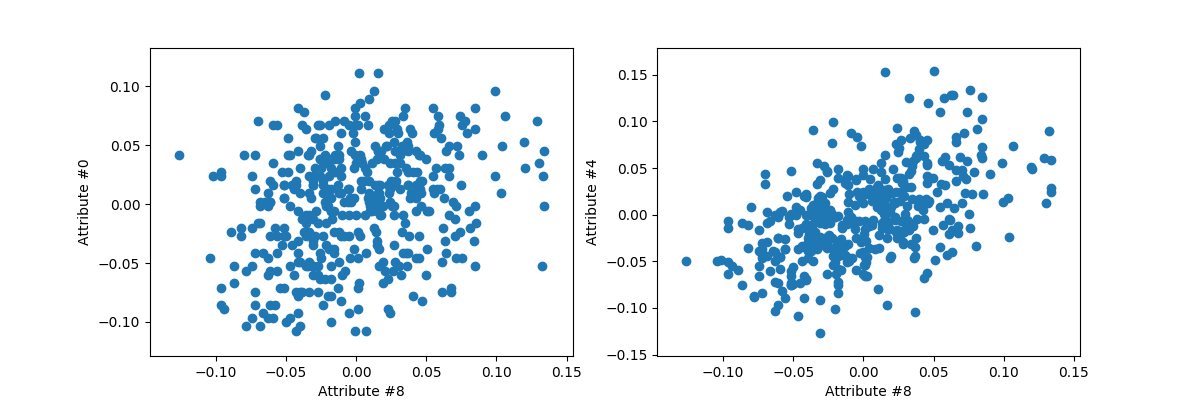
\includegraphics[scale=0.3]{correlation}
\captionof{figure}{}
\end{center}

\section{Solbility Prediction}

The accuracy of linear regression with L2 regularization on solubility dataset is illustrated in the figure below.
\begin{center}
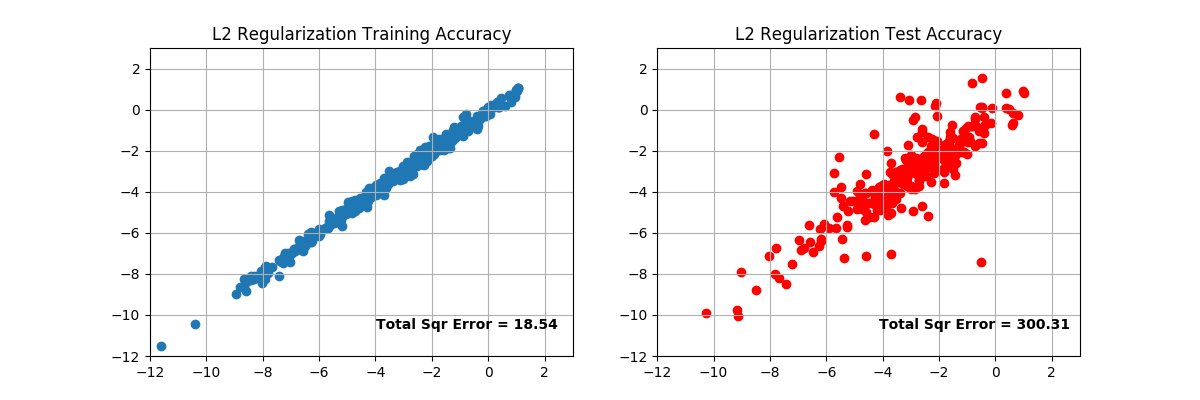
\includegraphics[scale=0.3]{tikhanov_solubility_acc} \\
\captionof{figure}{}
\end{center}

For Lasso, the models were slightly poorer on the training data but more accurate on the test set than L2 for all $\gamma$. The accuracy on test set and coefficients(non-zero only) are in the picture below. However, the total square error tends to increase together with the value of $\gamma$.
\begin{center}
\begin{tabular}{c}
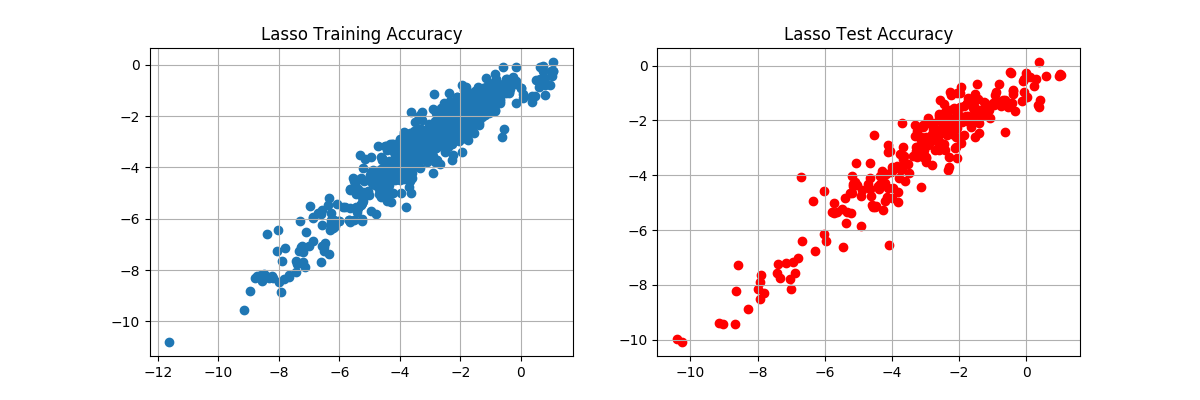
\includegraphics[scale=0.3]{lasso_solubility_acc}\\
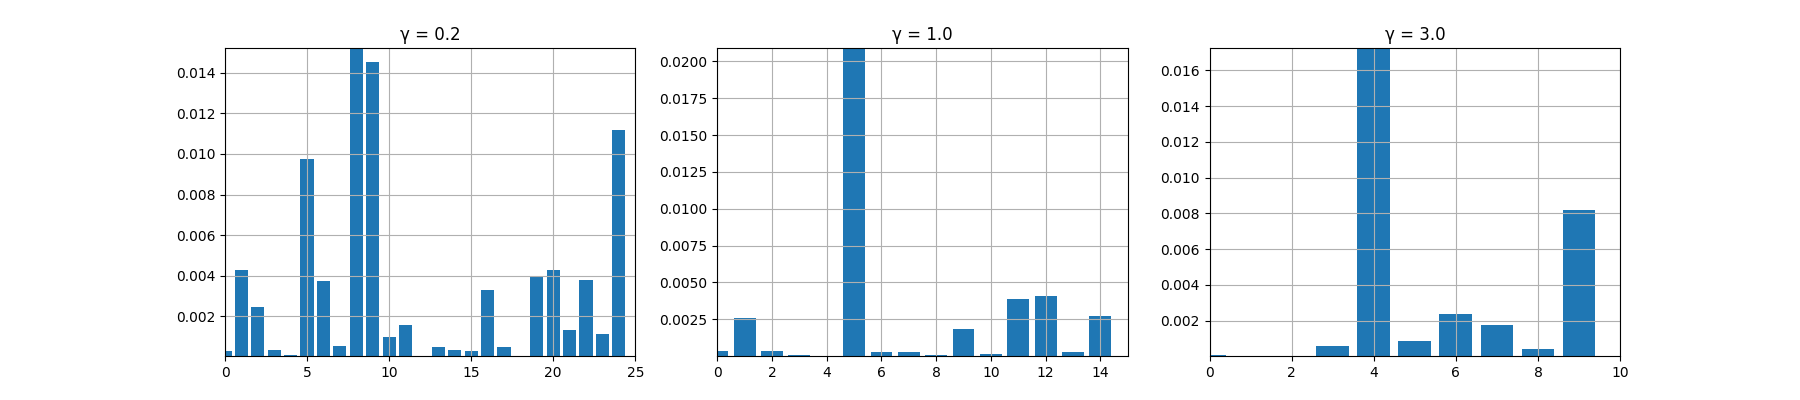
\includegraphics[scale=0.3]{lasso_solubility_coeff}\\
\end{tabular}
\captionof{figure}{}
\end{center}

To compare the result with the Artificial Neural Network method proposed by Huuskonen, 160 and 50 records are randomly selected from the whole dataset to be a training set and a test set respectively. The result compare to the ANN result in the journal is shown in the scatter plot below. From the picture, it can be seen that the technique proposed by Huuskonen perform better on the test set.
\begin{center}
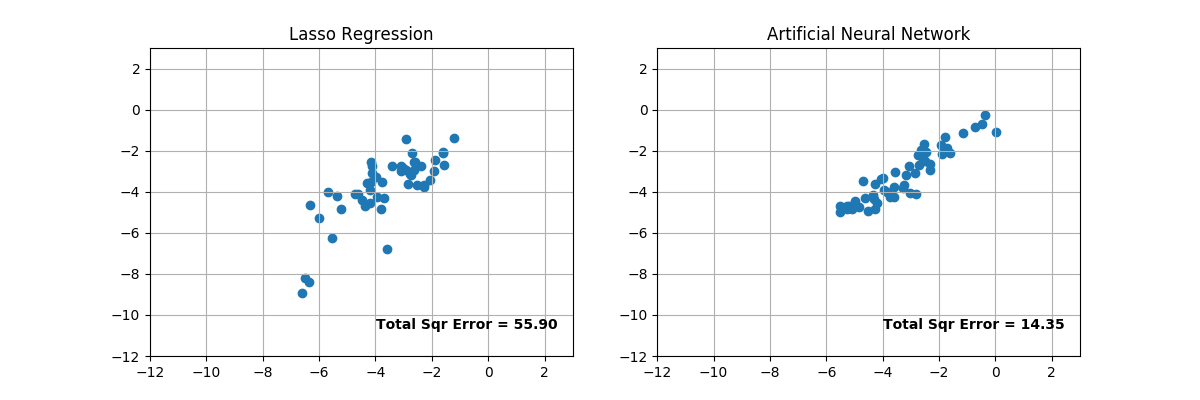
\includegraphics[scale=0.4]{lasso_ann_compare}
\captionof{figure}{}
\end{center}

\end{document}